\chapter{Resultados y discusión}
\thispagestyle{fancy}
% Resultados

Como se estableció en el capítulo anterior (sección \ref{sec:modelo}), el modelo considerado en el marco de la teoría relativista de campo medio contiene cinco parámetros libres: los tres acoplamientos mesón-nucleón $(g_\sigma/m_\sigma)$, $(g_\omega/m_\omega)$ y $(g_\rho/m_\rho)$, junto con los parámetros de autointeracción del mesón escalar $b$ y $c$. Estos parámetros determinan completamente la ecuación de estado de la materia nuclear y, consecuentemente, las propiedades macroscópicas de las estrellas de neutrones a través de las ecuaciones de estructura TOV (\ref{eq:tov}).

El ajuste de estos parámetros se realiza imponiendo que el modelo reproduzca las propiedades empíricas de la materia nuclear en saturación, descritas en la sección \ref{sec:saturacion}. Sin embargo, cada conjunto de parámetros que satisface estas restricciones nucleares produce una ecuación de estado diferente a altas densidades, generando predicciones distintas para las propiedades estelares observables como la masa máxima y el radio. Esta falta de unicidad en el espacio de parámetros refleja la incertidumbre en la extrapolación desde la densidad de saturación nuclear hacia los regímenes de densidad extrema presentes en el interior de las estrellas de neutrones.

El objetivo central de este capítulo es explorar sistemáticamente el espacio de parámetros del modelo, identificando los conjuntos que satisfacen las restricciones nucleares y que son consistentes con las observaciones astrofísicas actuales. Este análisis permite establecer relaciones entre los parámetros microscópicos del lagrangiano (\ref{eq:lagrangiano}) y las propiedades macroscópicas observables, permitiendo estudiar cómo las interacciones nucleares del modelo determinan la estructura de las estrellas de neutrones. En particular, se realiza la búsqueda del conjunto de parámetros que maximiza la masa estelar predicha, estableciendo límites superiores teóricos.

\clearpage
\section{Correlación entre Parámetros y Observables}

Partiendo del conjunto de parámetros \cite{glendenningCompactStarsNuclear2000}

\begin{equation}
\begin{aligned}
&A_\sigma = 12.684 \, m^2, &
&A_\omega = 7.148 \, m^2, \\
&A_\rho = 4.410 \, m^2, &
&b = 5.610\times10^{-3}, \\
&c = -6.986\times10^{-3}, & &
\label{eq:params_glendenning}
\end{aligned}
\end{equation}
	
se obtienen las propiedades nucleares y estelares

\begin{equation}
\begin{aligned}
&n_0 = 0.153 \, \text{fm}^{-3}, &
&\frac{B}{A} = -16.30 \, \text{MeV}, \\
&K_0 = 201.23 \, \text{MeV}, &
&a_\text{sym} = 32.54 \, \text{MeV}, \\
&L_0 = 79.63 \, \text{MeV}, & 
&M_\text{max} = 2.33 \, \masasol, \\
&R_{1.4} = 13.76 \, \text{km}, &
&C = 0.298. &
\label{eq:props_glendenning}
\end{aligned}
\end{equation}

Ya que los parámetros del modelo representan las intensidades físicas de las interacciones nucleares, es posible establecer correlaciones directas entre variaciones en estos parámetros y cambios en las propiedades nucleares y estelares. Por ejemplo, un aumento en el acoplamiento vectorial $A_\omega$ incrementa la repulsión entre nucleones, resultando en una disminución de la densidad de saturación $n_0$. Del mismo modo, un incremento en el acoplamiento isovectorial $A_\rho$ eleva la energía de simetría $a_\text{sym}$, afectando la composición protón-neutrón de la materia nuclear. Considerando variaciones de los parámetros alrededor de los valores en (\ref{eq:params_glendenning}), se observan las tendencias recopiladas en la figura \ref{fig:correlacionesparams}. Es necesario resaltar la independencia de $n_0$, $B/A$ y $K_0$ respecto a variaciones en $A_\rho$, lo cual es consistente con la interpretación física de este acoplamiento como responsable únicamente de las interacciones isovectoriales. Adicionalmente, parece relevante estudiar el espacio de parámetros $A_\sigma - A_\omega$, ya que ambos acoplamientos afectan todas las propiedades nucleares y estelares, sugiriendo una mayor influencia en la determinación de la ecuación de estado. Sobre el estudio del espacio de parámetros se profundiza en la siguiente sección.

\begin{figure}[h]
	\centering
	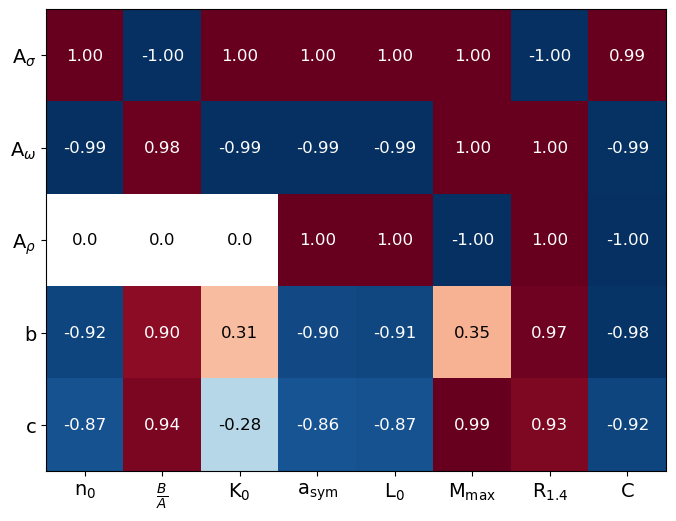
\includegraphics[width=0.7\linewidth]{Figuras/correlaciones_params}
	\caption[Correlaciones entre parámetros y observables]{Correlaciones cualitativas entre variaciones en los parámetros del modelo relativista de campo medio alrededor de los valores en (\ref{eq:params_glendenning}) y cambios en las propiedades nucleares y estelares. Valores cercanos a 1.0 indican una correlación positiva fuerte, mientras que valores cercanos a -1.0 indican una correlación negativa fuerte. Los valores intermedios reflejan correlaciones más débiles o nulas.}
	\label{fig:correlacionesparams}
\end{figure}


\section{Espacio de Parámetros}

La exploración del espacio de parámetros del modelo relativista de campo medio es un problema de optimización multidimensional bajo múltiples restricciones. El espacio completo está definido por los cinco parámetros libres: $A_\sigma$, $A_\omega$, $A_\rho$, $b$ y $c$. La metodología empleada para identificar conjuntos de parámetros físicamente aceptables consta de varias etapas sistemáticas.

Queremos identificar los conjuntos de parámetros que satisfacen las restricciones dentro de los márgenes experimentales. Estos conjuntos comprenden regiones del espacio de parámetros que son consistentes con las propiedades nucleares conocidas. Como puede evidenciarse en la figura \ref{fig:correlacionesparams}, los parámetros del modelo que influyen claramente en todas las propiedades nucleares y estelares son $A_\sigma$ y $A_\omega$, luego se decide realizar un barrido sistemático en el plano $A_\sigma - A_\omega$, mientras que los otros tres parámetros se ajustan para satisfacer las restricciones nucleares. De esta forma, para una elección particular de parámetros $b$ y $c$, los demás parámetros con influencia en el módulo de compresibilidad $K_0$, se busca la región del plano $A_\sigma - A_\omega$ que satisface las restricciones de densidad de saturación $n_0$ y de energía de enlace por nucleón $B/A$. Si los valores de $K_0$ dentro de esta región también cumplen la restricción impuesta, se procede a ajustar $A_\rho$ para satisfacer las restricciones de energía de simetría $a_\text{sym}$ y su pendiente $L_0$ sin afectar las otras propiedades nucleares, pues estas no dependen de $A_\rho$. Este procedimiento se repite para diferentes elecciones de los parámetros $b$ y $c$, explorando así el espacio de parámetros del modelo. La figura \ref{fig:flowchartmetodo} ilustra el flujo del método descrito. 

%\clearpage

%\begin{wrapfigure}{l}{0.38\textwidth}
%    \centering
%    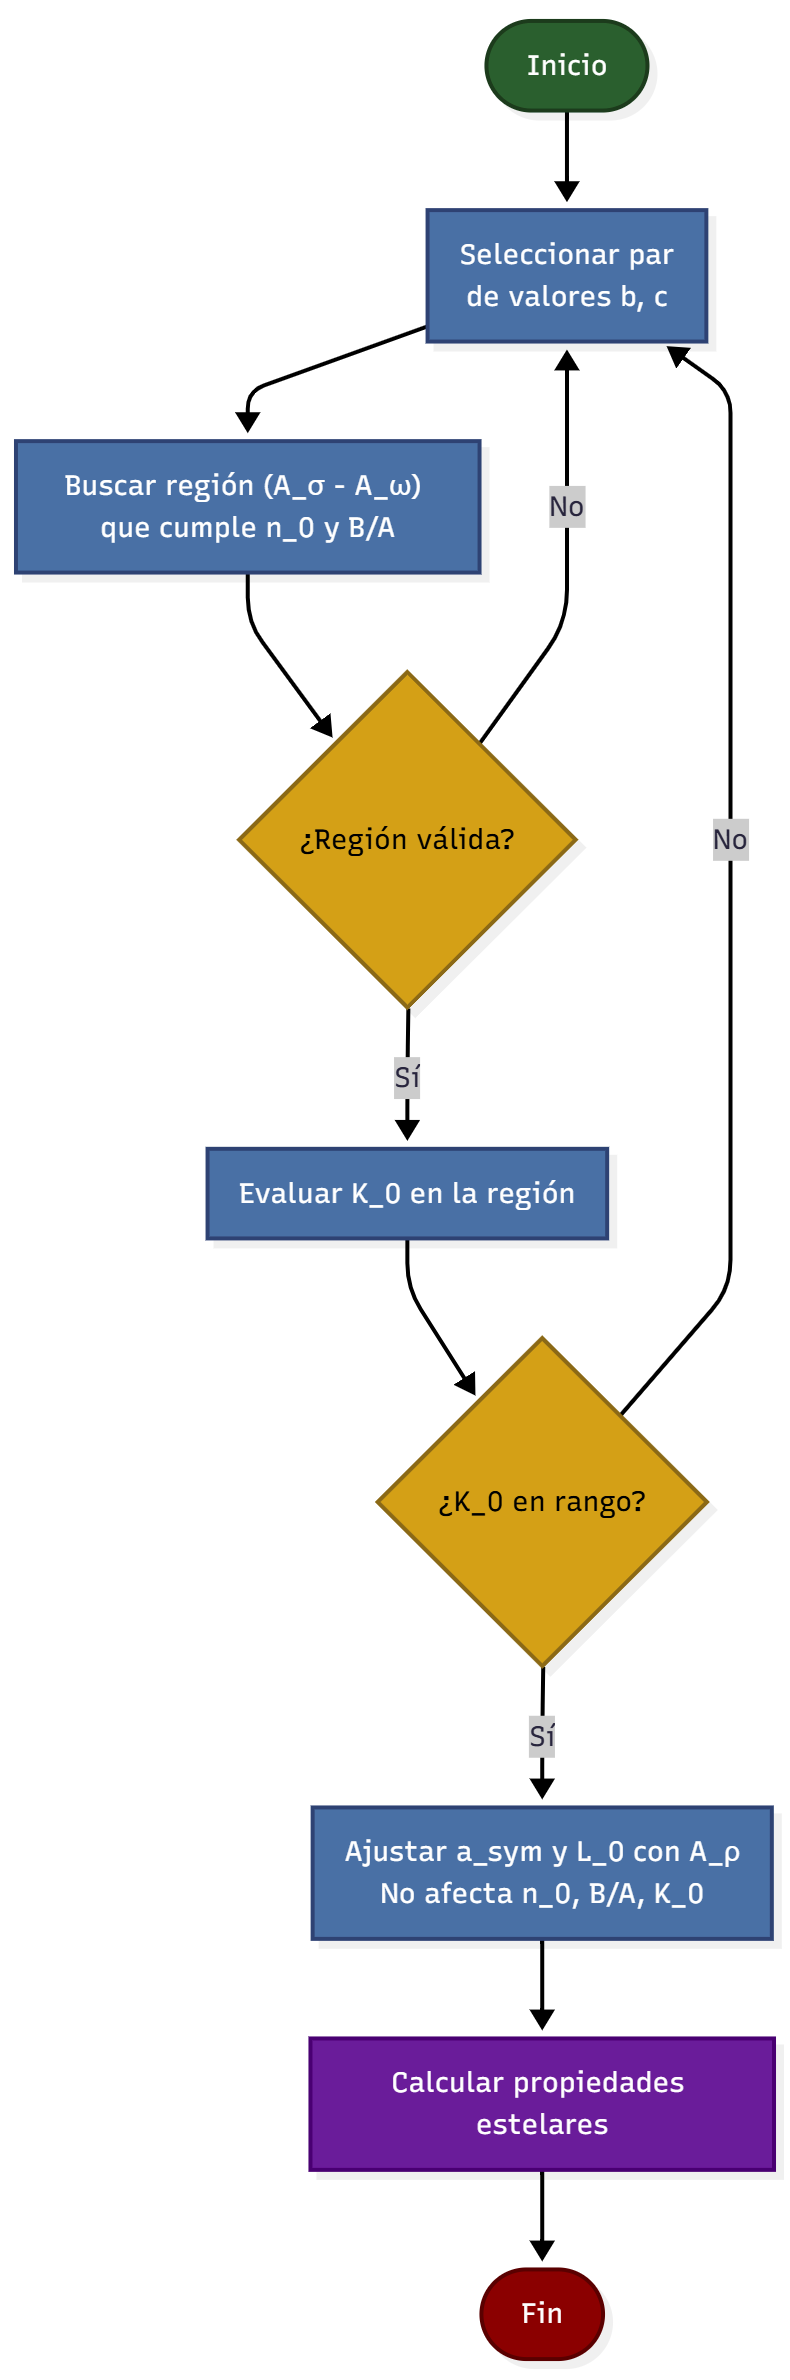
\includegraphics[width=\linewidth]{Figuras/flowchart_metodo}
%    \caption[Diagrama de flujo del método de exploración del espacio de parámetros]{Diagrama de flujo del procedimiento sistemático para explorar el espacio de parámetros del modelo relativista de campo medio.}
%    \label{fig:flowchartmetodo}
%\end{wrapfigure}

\begin{figure}
	\centering
	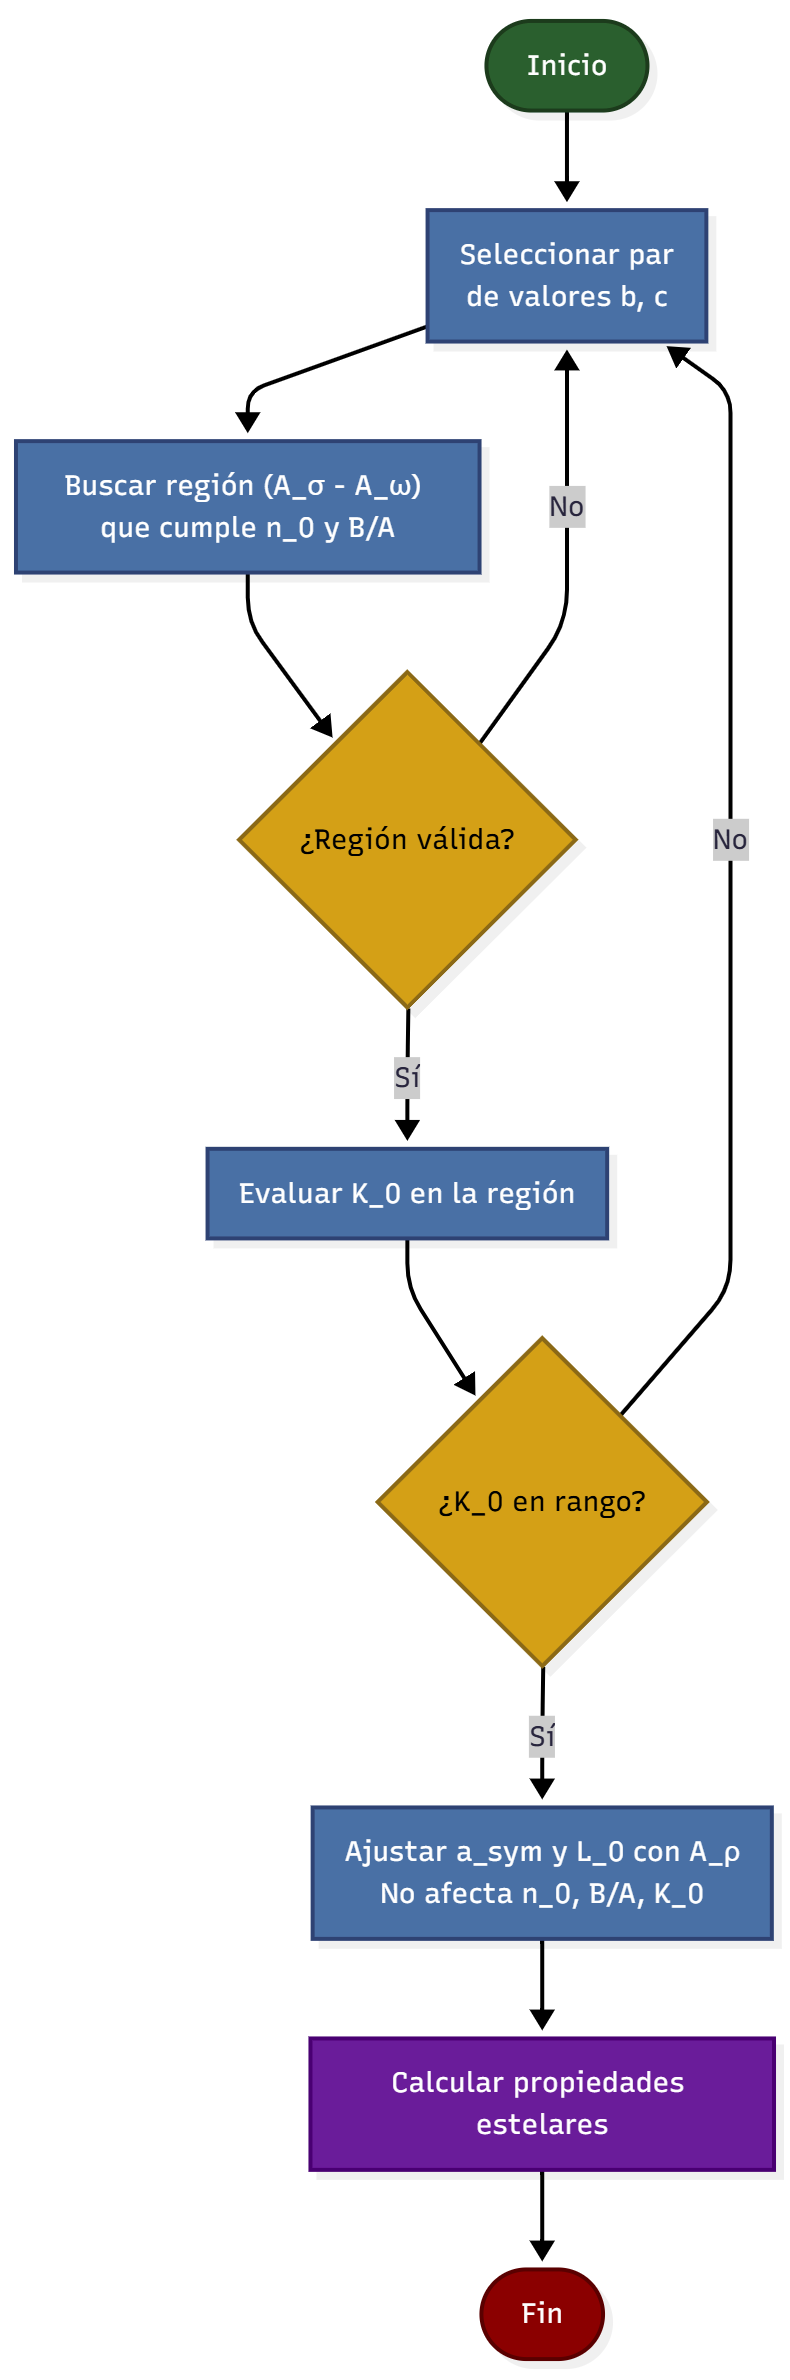
\includegraphics[width=.38\linewidth]{Figuras/flowchart_metodo}
	\caption[Diagrama de flujo del método de exploración del espacio de parámetros]{Diagrama de flujo del procedimiento sistemático para explorar el espacio de parámetros del modelo relativista de campo medio.}
	\label{fig:flowchartmetodo}
\end{figure}

Aplicando este método, se identifican múltiples conjuntos de parámetros que satisfacen las restricciones nucleares. Cada conjunto produce una ecuación de estado diferente a altas densidades, generando predicciones variadas para las propiedades estelares. Por ejemplo, tras realizar este proceso para un par de valores específicos de $b$ y $c$, se obtiene la región del plano $A_\sigma - A_\omega$ mostrada en la figura \ref{fig:region_nuclear_a}. Cada punto en esta región corresponde a un conjunto de parámetros que puede ser empleado para determinar las propiedades estelares resultantes, como la masa máxima y el radio de estrellas de neutrones. Además, si variamos los valores de $b$ y $c$ de modo que $K_0$ se mantenga dentro del rango aceptable, y ajustamos $A_\rho$ para cumplir las propiedades de simetría, obtenemos otras regiones válidas, como la mostrada en la figura \ref{fig:region_nuclear_b}. Esta nueva región tiene valores mayores de $A_\sigma$, $A_\omega$ y $c$, y valores menores de $A_\rho$ y $b$ en comparación con la región anterior.  

\begin{figure}[h]
    \centering
    \begin{subfigure}{\linewidth}
        \centering
        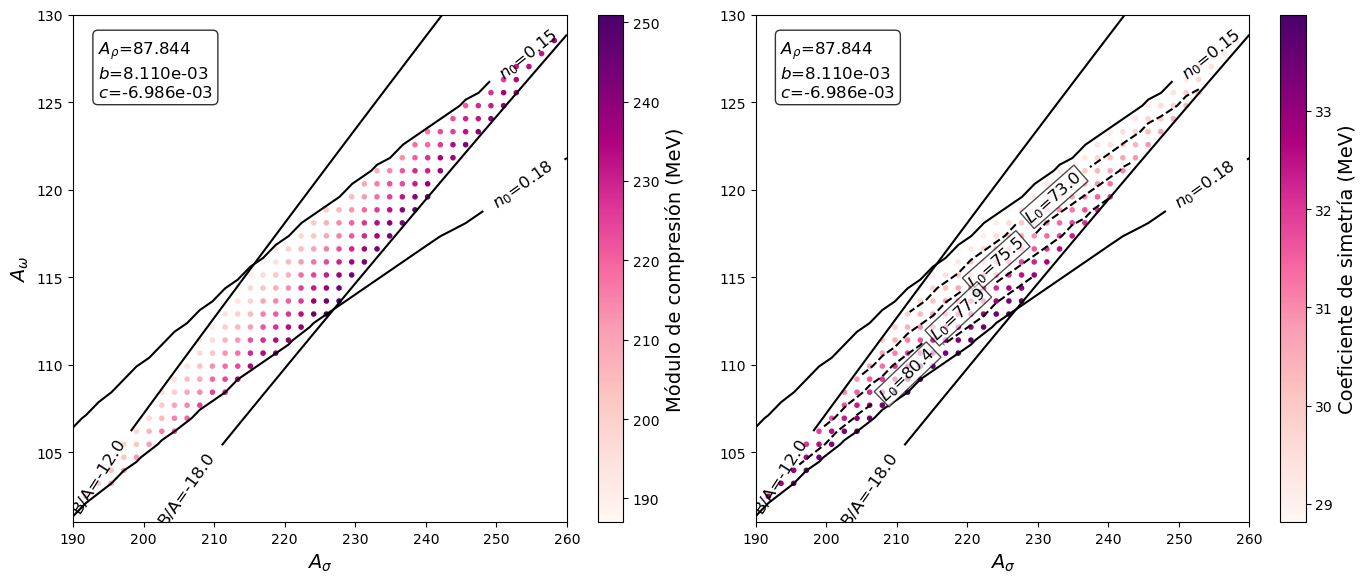
\includegraphics[width=0.85\linewidth]{Figuras/ejemplo_espacio_1}
        \caption{}
        \label{fig:region_nuclear_a}
    \end{subfigure}
    
    \begin{subfigure}{\linewidth}
        \centering
        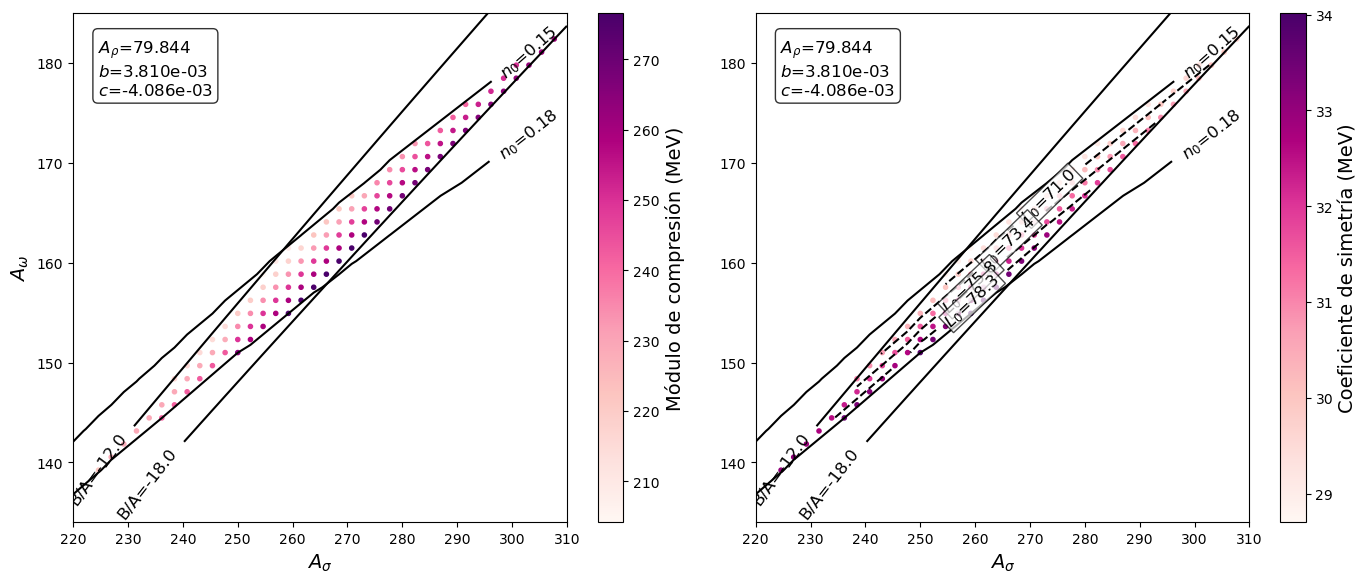
\includegraphics[width=0.85\linewidth]{Figuras/ejemplo_espacio_2}
        \caption{}
        \label{fig:region_nuclear_b}
    \end{subfigure}
    \caption[Regiones del espacio de parámetros que satisfacen las restricciones nucleares]{Región del espacio de parámetros que satisface las restricciones nucleares en el plano $A_\sigma - A_\omega$. (a) Conjunto de parámetros obtenido mediante la metodología descrita. (b) Región válida obtenida al variar $b$ y $c$ de (a) para mantener $K_0$ en el rango aceptable y ajustar $A_\rho$ para las propiedades de simetría. Las figuras muestran diferentes regiones del plano para facilitar la visualización.}
    \label{fig:region_nuclear}
\end{figure}

Siguiendo esta metodología, se consiguen diversos conjuntos de parámetros que cumplen las restricciones nucleares. Una vez obtenidos estos conjuntos, es posible calcular las propiedades estelares correspondientes, como la masa máxima $M_\text{max}$, la compacidad $C$ y el radio de estrellas de neutrones de masa $1.4 \, \masasol$, $R_{1.4}$. Para algunos conjuntos hallados, se muestran sus propiedades estelares en la figura \ref{fig:props_estelares}. Notamos que la masa máxima, la propiedad de mayor interés astrofísico, varía significativamente entre los diferentes conjuntos de parámetros, oscilando entre aproximadamente $1.9 \, \masasol$ y $2.3 \, \masasol$, y aumenta con valores mayores de $A_\sigma$ y $A_\omega$, al igual que el radio $R_{1.4}$, que toma valores entre $11.8 \, \text{km}$ y $13.3 \, \text{km}$. En cuanto a la compacidad $C$, se observa una tendencia similar respecto a los parámetros $A_\sigma$ y $A_\omega$, con valores que oscilan entre $0.278$ y $0.312$. Sin embargo, esta propiedad parece tener máximos locales en el plano que indican una dependencia más compleja con los parámetros del modelo.

\begin{figure}[h]
    \centering
    \begin{subfigure}{\linewidth}
        \centering
        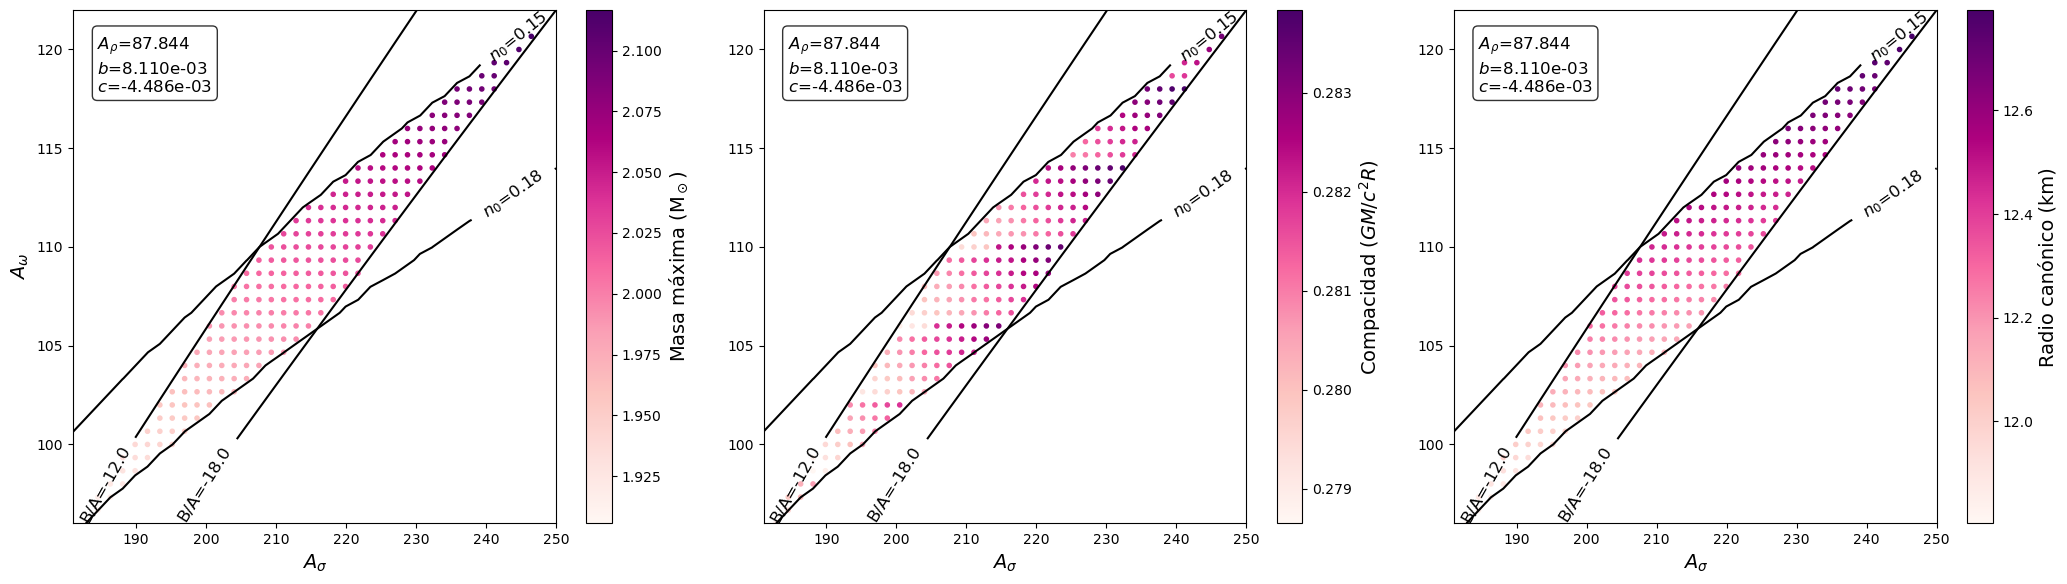
\includegraphics[width=0.99\linewidth]{Figuras/props_estelar_2}
        \caption{}
        \label{fig:props_estelar_2}
    \end{subfigure}
    
    \begin{subfigure}{\linewidth}
        \centering
        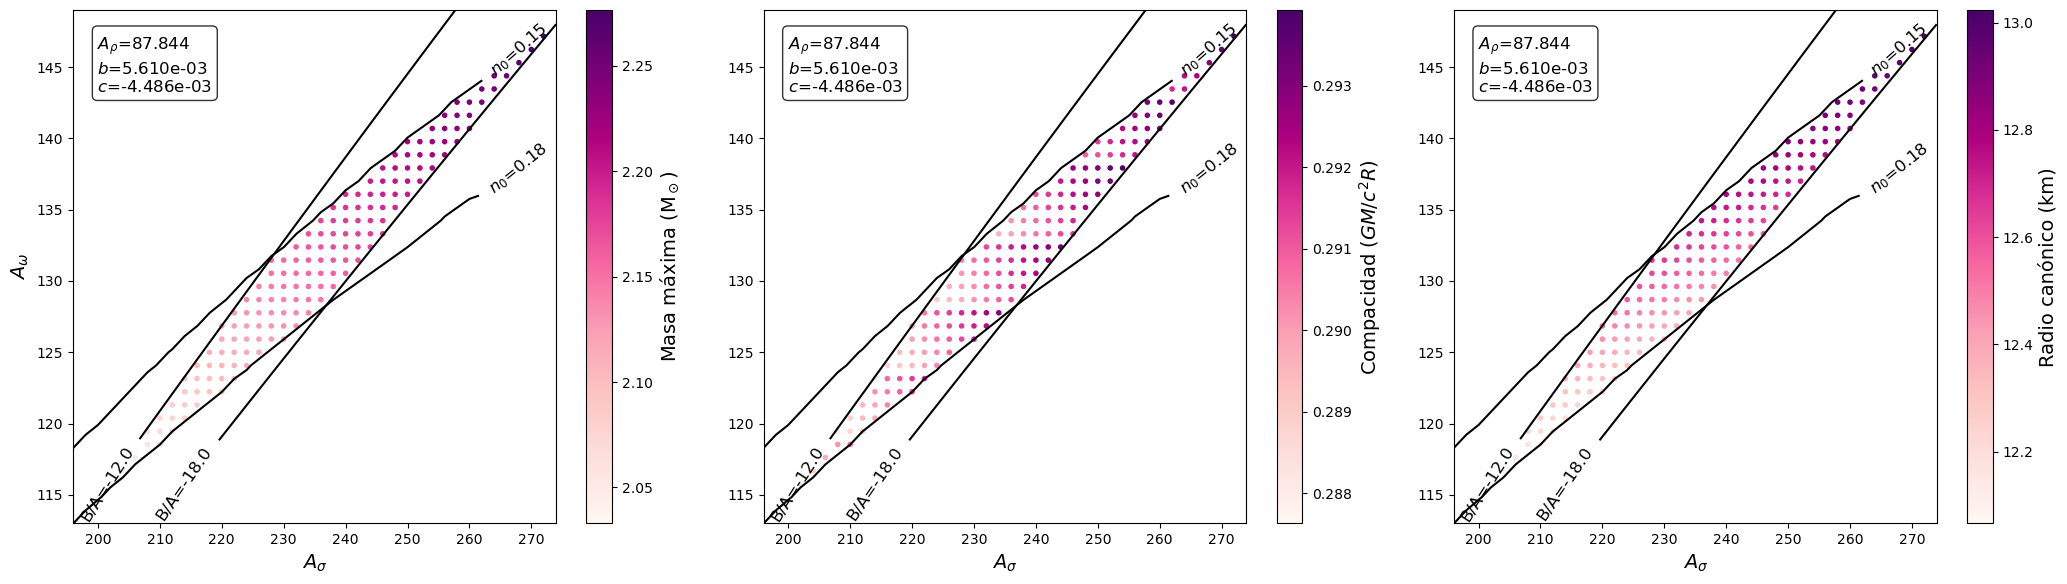
\includegraphics[width=0.99\linewidth]{Figuras/props_estelar_1}
        \caption{}
        \label{fig:props_estelar_1}
    \end{subfigure}
    
    \begin{subfigure}{\linewidth}
        \centering
        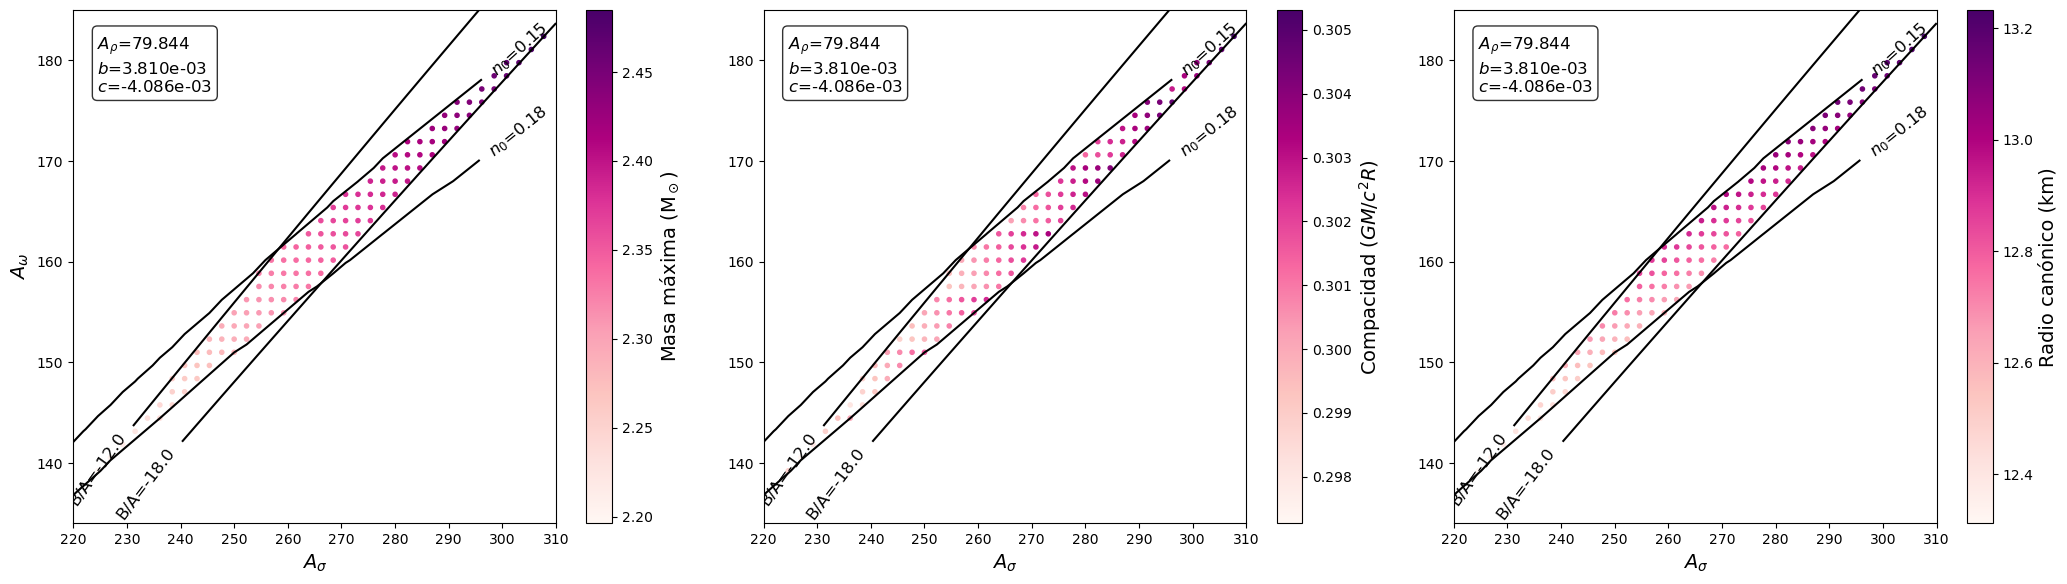
\includegraphics[width=0.99\linewidth]{Figuras/props_estelar_3}
        \caption{}
        \label{fig:props_estelar_3}
    \end{subfigure}
    
    \begin{subfigure}{\linewidth}
        \centering
        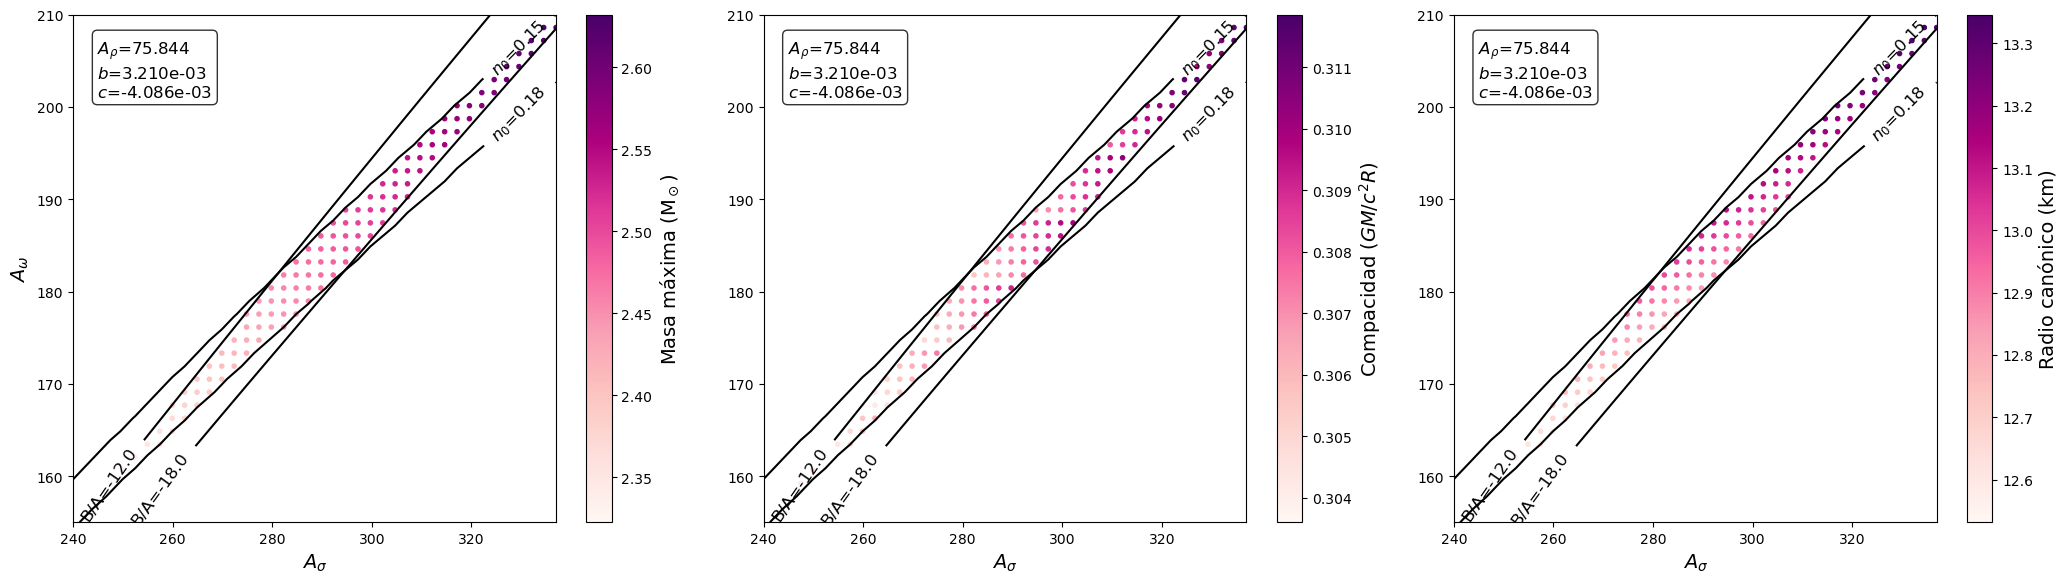
\includegraphics[width=0.99\linewidth]{Figuras/props_estelar_4}
        \caption{}
        \label{fig:props_estelar_4}
    \end{subfigure}
    \caption[Propiedades estelares para diferentes conjuntos de parámetros]{Propiedades estelares obtenidas para diferentes conjuntos de parámetros que satisfacen las restricciones nucleares. Las figuras muestran diferentes regiones del plano $A_\sigma - A_\omega$ para facilitar la visualización.}
    \label{fig:props_estelares}
\end{figure}
\clearpage


\subsection{Masa Máxima}

La búsqueda del conjunto de parámetros que maximiza la masa estelar predicha es un objetivo central del análisis. Este conjunto establece el límite superior teórico para la masa de estrellas de neutrones dentro del marco del modelo considerado, y su comparación con las observaciones de estrellas masivas como las mencionadas en la sección \ref{sec:obsNS} permite evaluar si el modelo es capaz de explicar las configuraciones estelares más extremas observadas.

\begin{figure}[h]
	\centering
	\begin{subfigure}{\linewidth}
		\centering
		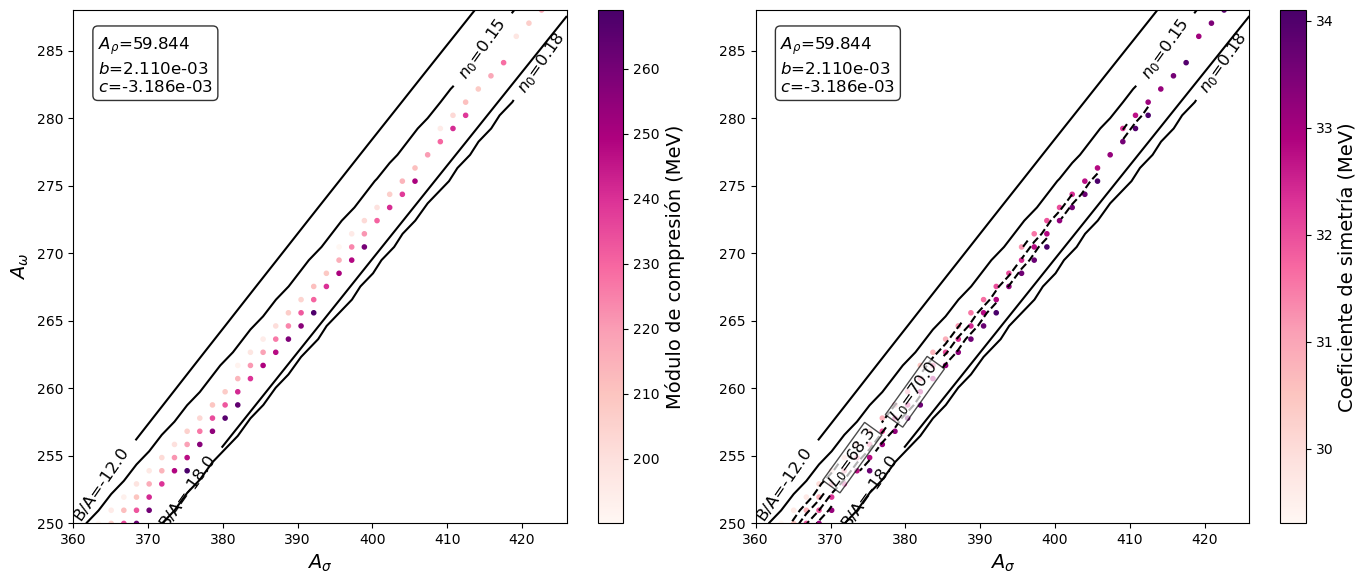
\includegraphics[width=0.85\linewidth]{Figuras/ejemplo_espacio_maxmass}
		\caption{}
		\label{fig:ejemplo_espacio_maxmass}
	\end{subfigure}
	
	\begin{subfigure}{\linewidth}
		\centering
		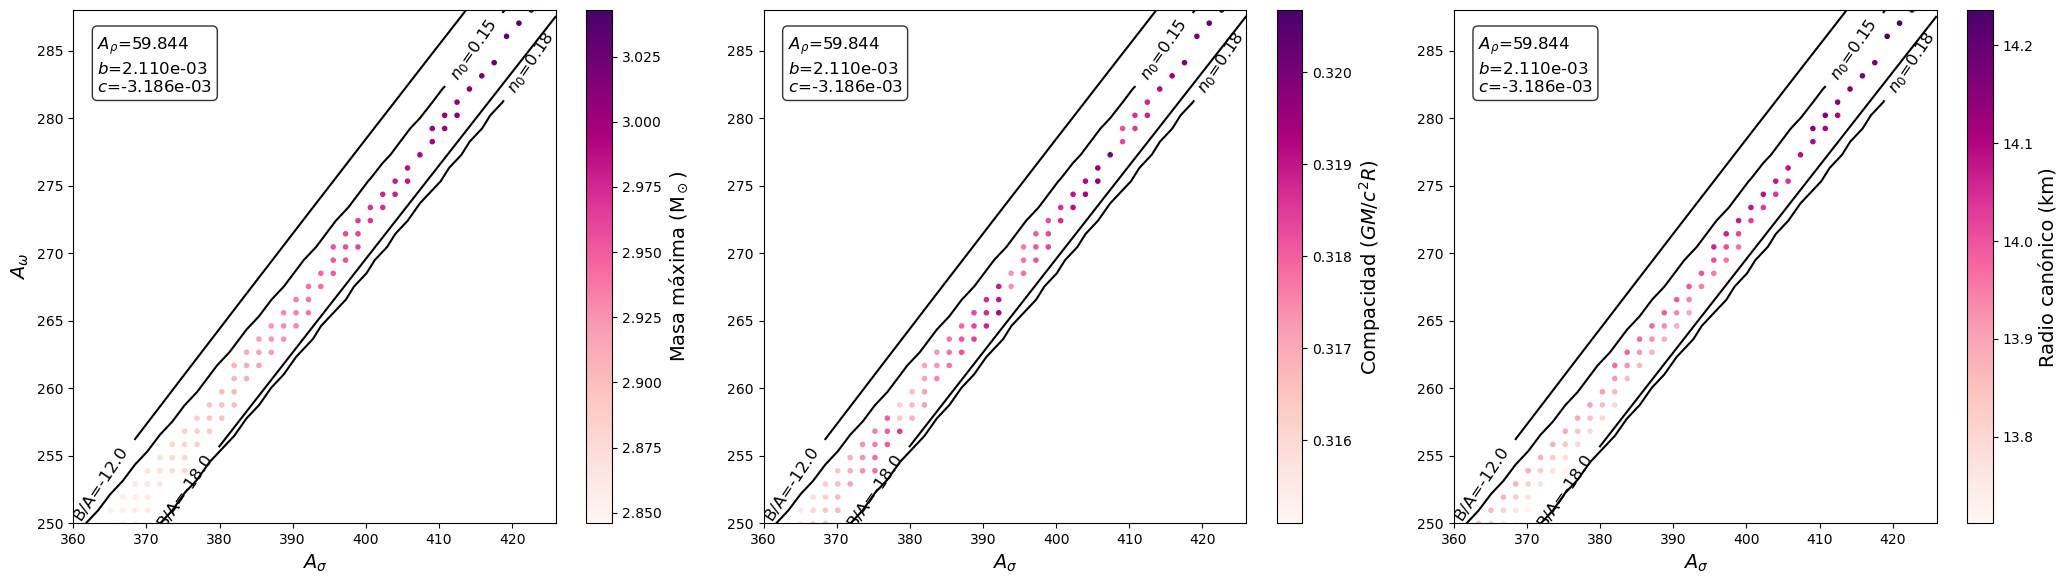
\includegraphics[width=0.99\linewidth]{Figuras/props_estelar_maxmass}
		\caption{}
		\label{fig:props_estelar_maxmass}
	\end{subfigure}
	\caption[Región de masa máxima en el espacio de parámetros]{Región del espacio de parámetros que maximiza la masa estelar predicha. (a) Propiedades nucleares para la región de parámetros que produce la mayor masa máxima. (b) Propiedades estelares correspondientes: masa máxima $M_\text{max}$, compacidad $C$ y radio $R_{1.4}$ para configuraciones en esta región.}
	\label{fig:max_mass}
\end{figure}

La región de mayores masas obtenidas para este modelo mediante la metodología descrita, así como sus propiedades nucleares y estelares, se muestra en la figura \ref{fig:max_mass}. En este estudio, se logró obtener una masa máxima de $M_\text{max} = 3.04 \, \masasol$, superando ampliamente el límite observado en radiación electromagnética de $2.35 \, \masasol$ para PSR J0952-0607 \cite{romaniPSRJ09520607Fastest2022}. Esto indica que el modelo relativista de campo medio, con los parámetros adecuados, puede reproducir estrellas de neutrones extremadamente masivas, siendo un marco teórico consistente con las observaciones astrofísicas más exigentes. Más aún, no queda claro que la región de parámetros de mayor masa encontrada en este estudio sea el límite absoluto dentro del modelo, por lo que futuros estudios y técnicas de optimización más avanzadas podrían revelar conjuntos de parámetros que produzcan masas aún mayores, sin contradecir las restricciones nucleares impuestas. Correspondientemente, se logra una compacidad máxima de $C = 0.32$ y un radio máximo de $R_{1.4} = 14.24 \, \text{km}$ para estrellas de masa $1.4 \, \masasol$ en esta región de parámetros.

\subsection{Comparación de Regiones}

Las regiones de parámetros mostradas en las figuras \ref{fig:region_nuclear}, \ref{fig:props_estelares} y \ref{fig:max_mass} representan diferentes áreas del espacio de parámetros que satisfacen las restricciones nucleares y producen diversas propiedades estelares. Es relevante comparar estas regiones para entender cómo las variaciones en los parámetros afectan las predicciones del modelo. En la figura \ref{fig:comparacion_regiones} se presenta una comparación directa entre las regiones que satisfacen las restricciones nucleares y las masas máximas que producen. Como notamos anteriormente, el aumento en los acoplamientos $A_\sigma$ y $A_\omega$ conduce a un incremento en la masa máxima predicha. Más aún, para mantener las propiedades de simetría dentro de los rangos aceptables, es necesario reducir el acoplamiento isovectorial $A_\rho$ al aumentar $A_\sigma$ y $A_\omega$. Esto puede explicarse por la necesidad de compensar el efecto de los acoplamientos escalares y vectoriales que tienden a aumentar la energía, requiriendo una disminución en la contribución isovectorial. Esta comparación resalta la interdependencia entre los parámetros del modelo y las propiedades estelares, por lo que es importante considerar estas relaciones al ajustar el modelo a observaciones astrofísicas.

\begin{figure}[h]
    \centering
    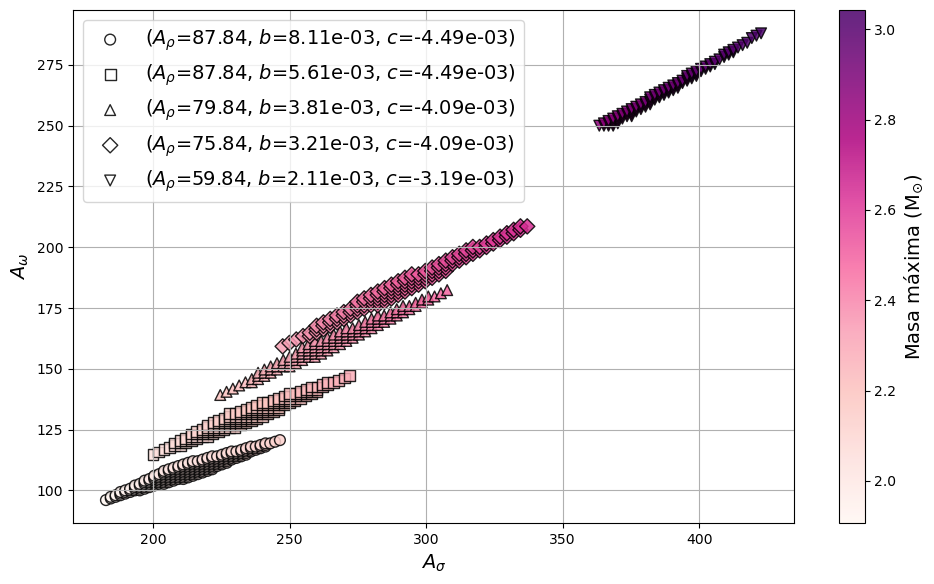
\includegraphics[width=0.7\linewidth]{Figuras/comparacion_regiones}
    \caption[Comparación de regiones en el plano $A_\sigma$ - $A_\omega$]{Comparación de las regiones del plano de parámetros $A_\sigma$ - $A_\omega$ que satisfacen las restricciones nucleares y las masas máximas que producen.}
    \label{fig:comparacion_regiones}
\end{figure}